\section{Acceptance correction}
\label{sec:swave:meas:ac}

The distribution of \BdToKpimm events in terms of \psq, \qsq and \ctk which pass the selection is not entirely 
representative of the distribution from all \BdToKpimm decays.
This is because the selection of \BdToKpimm candidates introduces an acceptance effect 
in all three of these variables.
The mass model used to analyse the distribution of \BdToKpimm events describes the 
fundamental distribution of events requiring that any acceptance effect must be corrected for.

The acceptance for \BdToKpimm is given by the inverse of the efficiency to select \BdToKpimm events,
\begin{align}
\epsilon(\psq,\qsq,\ctk) = \frac{ S(\psq,\qsq,\ctk) }{ G(\psq,\qsq,\ctk) } \, ,
\end{align}
where the efficiency can be calculated by considering the number of simulated events which pass the selection ($S$)
when compared to the number of simulated events at the generator level ($G$) .

Following the work in Section~\ref{sec:kstmm:ac}, the acceptance is evaluated
 using simulated \BdToKpimm events generated uniformly across the phase space.
For phase space simulated events, the \qsq region considered is from 0.1 to 19 \gevgevcccc 
and the \psq region is from the \kpi threshold (0.4) to 1.44 \gevgevcccc.
%The limited \psq window means that the statistics of the phase space generated \BdToKpimm sample 
%are in not as great as the statistics of the \BdToKstmm simulation sample used in Sec~\ref{sec:kstmm:ac}, 
%which corresponds to a reduction in the accuracy on the efficiency correction. 

The distribution of phase space simulated events at generator level for \psq and \qsq are given in Fig.~\ref{fig:swave:ac:genlevel}.
\begin{figure}[tbp]
\centering
\subfigure[]{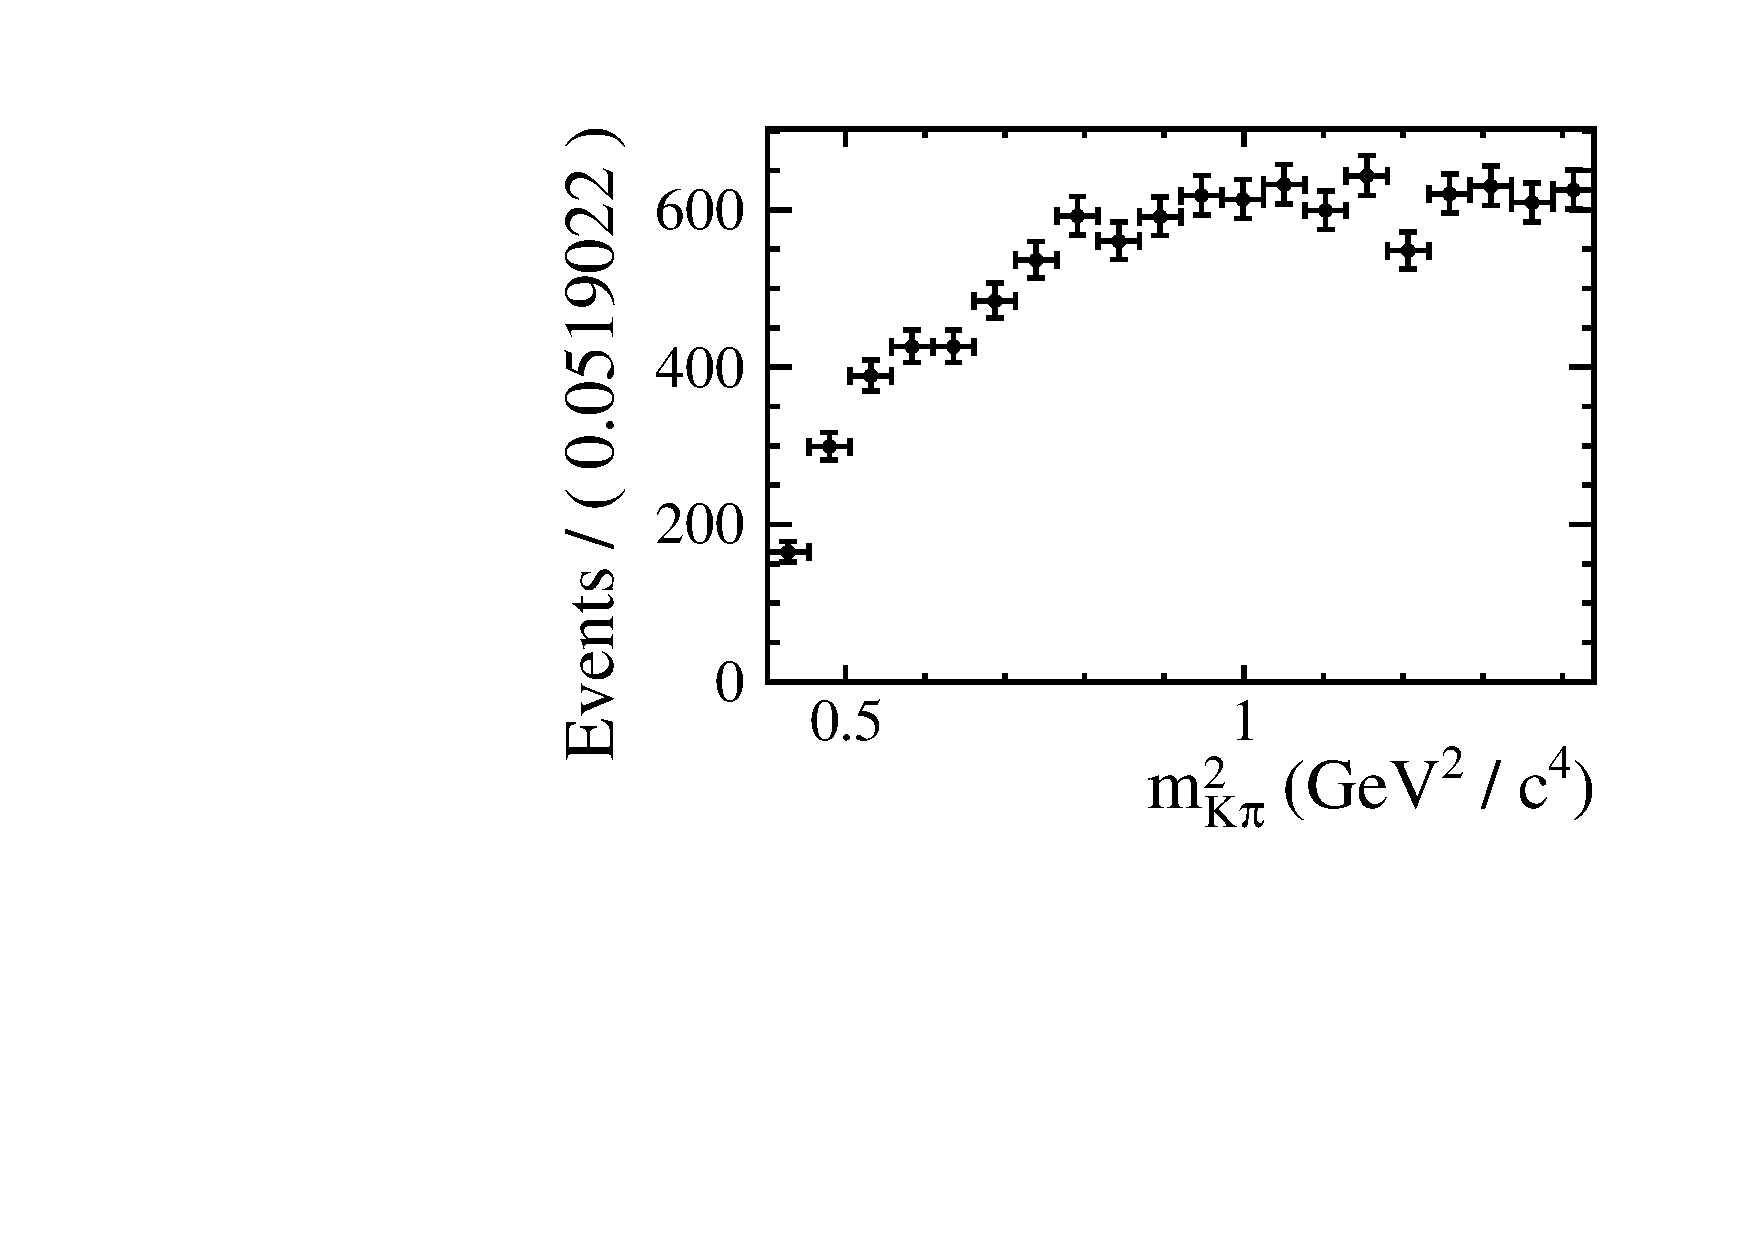
\includegraphics[width=0.48\columnwidth,page=1]{chapter7/figs/ac/fitkpieff_sq_dist_plots.pdf}}
\subfigure[]{\includegraphics[width=0.48\columnwidth,page=2]{chapter7/figs/ac/fitkpieff_sq_dist_plots.pdf}}
\caption[ The distribution of phase space \BdToKpill simulated events at generator level
as a function of (a) \psq and (b) \qsq.   ]
{ The distribution of phase space \BdToKpill simulated events at generator level
as a function of (a) \psq and (b) \qsq.  %and (c) \ctk. 
%The distribution of events increases from the threshold for the low \psq region considered.
%There is a small increase from threshold but an overall decrease in events across \qsq.
~\label{fig:swave:ac:genlevel} }
\end{figure}
%It can be seen that the region of \psq considered is sufficienctly small
%that the phase space is still increasing from threshold in this region.
%The distribution of events in \qsq covers almost the full phase space, 
%both increasing from the lower bound of 0.1.0\gevgevcccc and then decreasing to the upper bound of 19\gevgevcccc.
After the selection has been applied, along with the data-simulation corrections, there are around 
ten thousand simulated phase space events left, giving a total efficiency  for \BdToKpimm of around $0.1\%$.
In order to make maximum use of the simulation statistics, the efficiency was checked for correlations between the 
kinematic variables with the aim of factorising the efficiencies into one dimensional functions.

\subsection{Efficiency in terms of \psq, \qsq and \ctk}

The efficiency to select \BdToKpimm events in terms of \psq, \qsq and \ctk is shown in 
Fig.~\ref{fig:swave:ac:eff1D}.
\begin{figure}[tbp]
\centering
\subfigure[]{\includegraphics[width=0.32\columnwidth,page=2]{chapter7/figs/ac/effplots1D.pdf}}
\subfigure[]{\includegraphics[width=0.32\columnwidth,page=4]{chapter7/figs/ac/effplots1D.pdf}}
\subfigure[]{\includegraphics[width=0.32\columnwidth,page=5]{chapter7/figs/ac/effplots1D.pdf}}
\caption{ The efficiency as a function of (a) \psq, (b) \qsq  and (c) \ctk for phase space simulated \BdToKpimm events. 
%There are between 10 and 100 events which pass the \kpimm candidate selection  in each bin.  
~\label{fig:swave:ac:eff1D} }
\end{figure}
It is possible to see the drop at high \ctk coming from the asymmetric \kaon and \pion acceptance.
There is also a drop in efficiency for low \psq values and high \qsq values.
The efficiency in each of the two dimensional distributions (\psq v.s. \qsq, \psq v.s. \ctk and \qsq v.s. \ctk) is shown in 
Fig.~\ref{fig:swave:ac:eff2D}.
\begin{figure}[tbp]
\centering
\subfigure[]{\includegraphics[width=0.32\columnwidth,page=2]{chapter7/figs/ac/effplots2D.pdf}}
\subfigure[]{\includegraphics[width=0.32\columnwidth,page=4]{chapter7/figs/ac/effplots2D.pdf}}
\subfigure[]{\includegraphics[width=0.32\columnwidth,page=6]{chapter7/figs/ac/effplots2D.pdf}}
\caption[ The efficiency as a function of (a) \psq and \qsq, (b) \psq and \ctk and (c) \qsq and \ctk 
for phase space simulated \BdToKpimm events.]
{ The efficiency as a function of (a) \psq and \qsq, (b) \psq and \ctk and (c) \qsq and \ctk 
for phase space simulated \BdToKpimm events. There are between 10 and 100 events which pass the \kpimm candidate selection 
 in each bin.  ~\label{fig:swave:ac:eff2D} }
\end{figure}
%It is possible to see the drop at high \ctk across \psq and \qsq coming from the asymmetric \kaon and \pion acceptance.
There is an asymmetric effect in \ctk in both the low and high \qsq regions due to the momentum difference between the kaon and pion
in the lab frame. 
%There is also a drop in efficiency for both low \psq and high \qsq values.
There is also a correlation between the efficiency in \psq and \ctk , changing between low and high values of \psq at high \ctk values.
The detailed examination of the P-wave efficiency in Section~\ref{sec:kstmm:ac} shows that there is a correlation between 
the efficiency in \ctk and \qsq.
The projected efficiencies in different regions of \psq and \qsq are is shown in Figure~\ref{fig:swave:meas:corr}.
\begin{figure}[tbp]
\centering
\subfigure[]{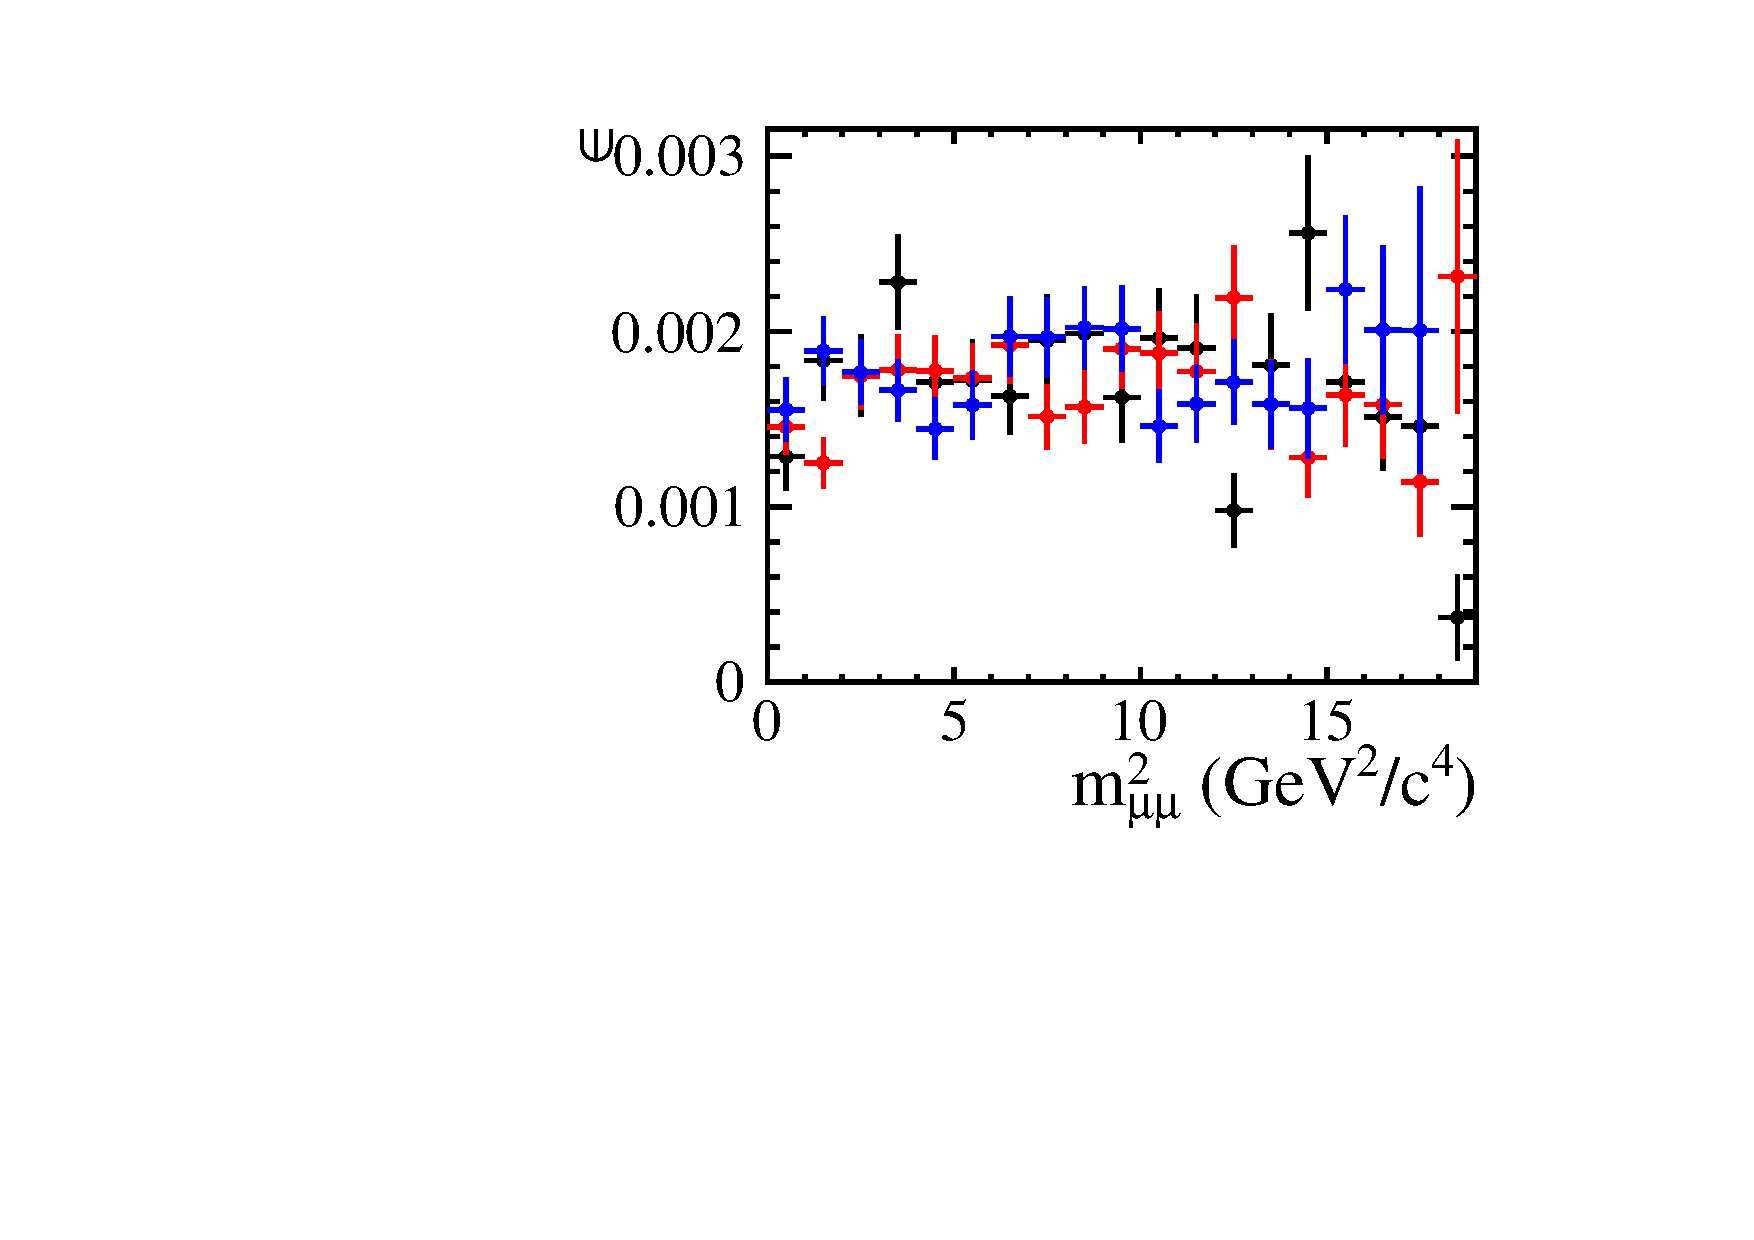
\includegraphics[width=0.32\columnwidth]{chapter7/figs/ac/effplots2D_proj_x.pdf}}
\subfigure[]{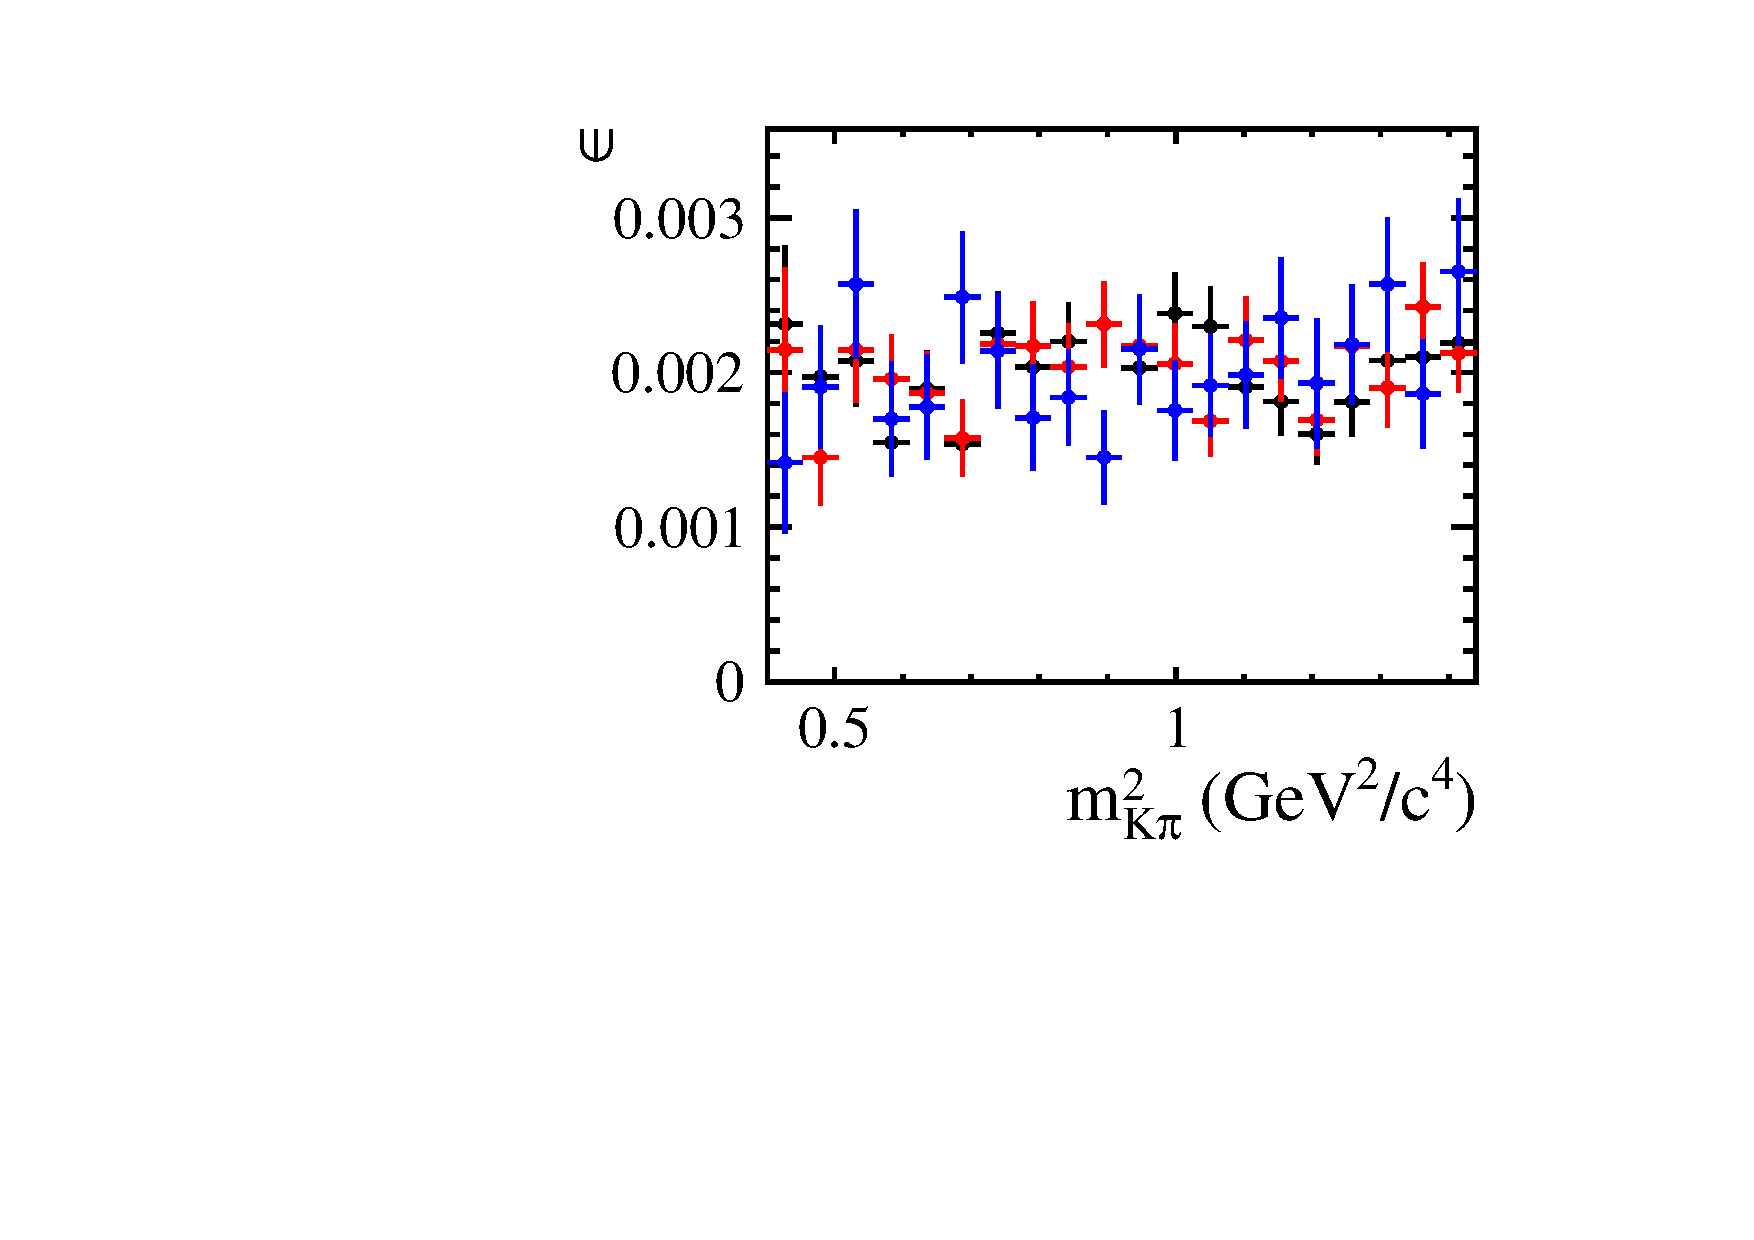
\includegraphics[width=0.32\columnwidth]{chapter7/figs/ac/effplots2D_proj_y.pdf}}
\caption{ The projected efficiency for (a) \psq in 1 \gevgevcccc wide bins around \qsq values of 5, 10 and 15 \gevgevcccc and (b) 
\qsq in 0.02 \gevgevcccc wide bins at \psq values of 0.49, 0.64 and 0.81 \gevgevcccc. 
The efficiency projections was tested using the Kolmogorov-Smirnov test and found to be compatible.
~\label{fig:swave:meas:corr}}
\end{figure}
The compatibility of the different efficiency projections was tested using the Kolmogorov-Smirnov test~\cite{KSTEST}.
No extreme $p$-values were found which implies that the efficiency projections are compatible with coming from the same parent efficiency distribution.
This shows that in the limit of the simulation statistics used, there is no correlation between the efficiency in \psq and \qsq.

In order to examine how the \ctk efficiency changes in terms of \psq, the efficiency of \BdToKpimm events was modelled in three bins of \psq. 
These are the regions from threshold to 0.64\gevgevcccc, the P-wave mass window from 0.64 to 1.00\gevgevcccc and above the P-wave from 1.00 to 1.44\gevgevcccc.
The efficiency as a function of \ctk for each of these regions is shown in Fig.~\ref{fig:swave:meas:ctk:eff}.
\begin{figure}[tbp]
\centering
\subfigure[]{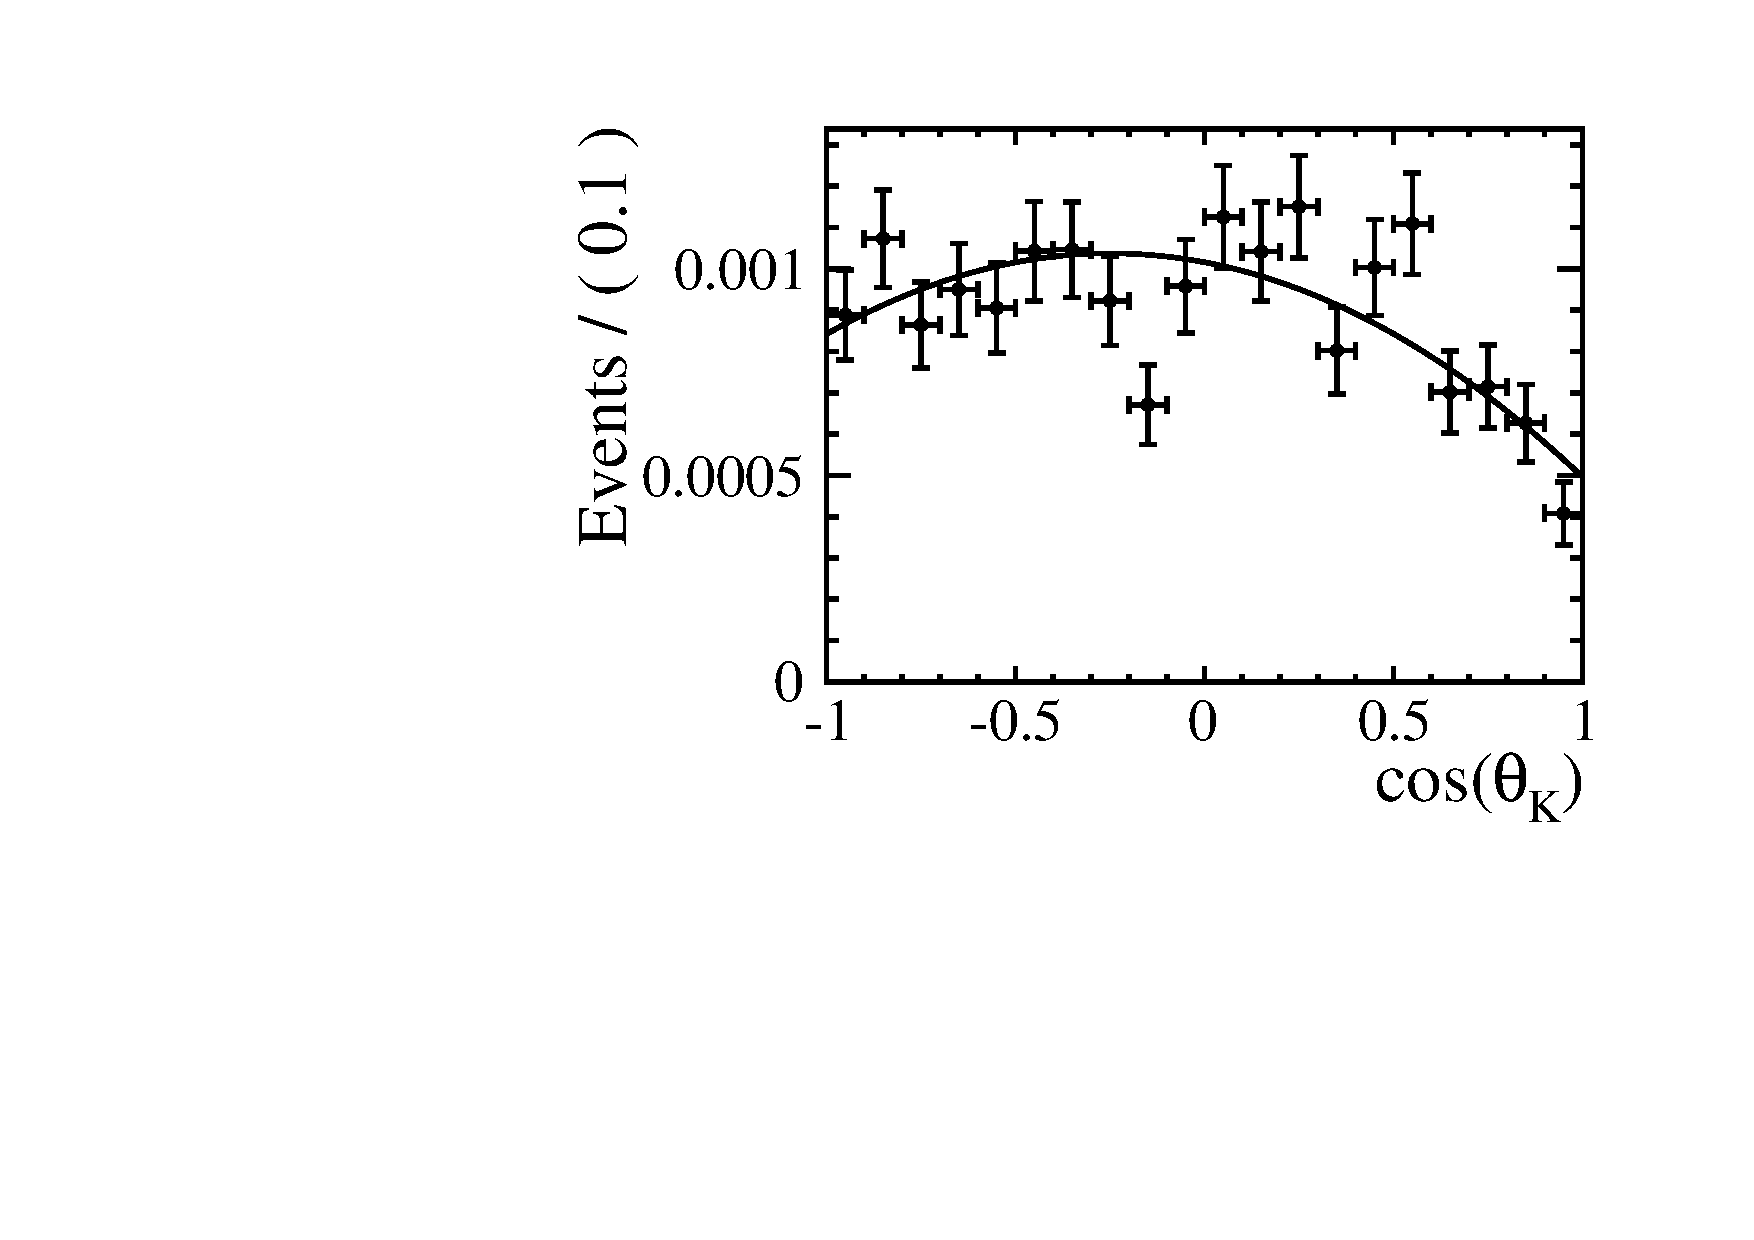
\includegraphics[width=0.32\columnwidth,page=1]{chapter7/figs/ac/fitplots_ctk.pdf}}
\subfigure[]{\includegraphics[width=0.32\columnwidth,page=2]{chapter7/figs/ac/fitplots_ctk.pdf}}
\subfigure[]{\includegraphics[width=0.32\columnwidth,page=3]{chapter7/figs/ac/fitplots_ctk.pdf}}
\caption[ The efficiency as a function of \ctk for phase space simulated \BdToKpimm events.  ]
{The efficiency as a function of \ctk for phase space simulated \BdToKpimm events.
 The low \mkpi region below 0.64\gevgevcccc is shown in (a), the region around the P-wave resonance in (b) and the high \mkpi region between 1.00 to 1.44\gevgevcccc in (c).
The efficiency is fitted with a second order Chebychev polynomial (the \textcolor{black}{black} curve) showing the parametrised efficiency in each \psq bin. 
~\label{fig:swave:meas:ctk:eff} }
\end{figure}
It is possible to see a change in the shape of the efficiency between the different \psq bins, 
but there are insufficient simulated statistics to provide an accurate correction in \ctk.
%Each of the fitted Chebychev polynomials are compatible to within $2\sigma$, allowing the efficiency in the P-wave region
%to be applied to the low and high \psq regions.
Since the statistics of the \BdToKpimm simulation sample are insufficient to correct in \psq, \qsq and \ctk,
\ctk must be integrated out.
However, the integration over \ctk contributes to a source of systematic uncertainty.

The event-by-event acceptance correction for the \BdToKpimm events is obtained by the calculating the values for the 
polynomial models for the \psq and \qsq efficiencies,
\begin{align}
\epsilon(\psq,\qsq) = P(\psq; p_0, p_1, p_2, p_3) \times P(\qsq; q_0, q_1, q_2, q_3) \, ,
\end{align}
and the weight of each event to correct for the acceptance is given by the inverse efficiency, 
\begin{align}
\omega(\psq,\qsq) = 1 / \epsilon(\psq,\qsq) \, .
\end{align}

\subsection{Validation}

The acceptance correction can be checked to first order by comparing the distribution of re-weighted events 
to the expected distribution of events at generator level
Following Section~\ref{sec:kstmm:ac}, the selected simulation used to calculate $S(\psq,\qsq)$ 
is re-weighted and compared to the distribution of generator level events used to calculate $G(\psq,\qsq)$.
The distributions of simulation can be seen in Fig.~\ref{fig:swave:ac:validation}.
\begin{figure}[tbp]
\centering
\subfigure[]{\includegraphics[width=0.32\columnwidth,page=4]{chapter7/figs/ac/validation_ac_1D.pdf}}
\subfigure[]{\includegraphics[width=0.32\columnwidth,page=3]{chapter7/figs/ac/validation_ac_1D.pdf}}
%\subfigure[]{\includegraphics[width=0.32\columnwidth,page=5]{chapter7/figs/ac/validation_ac_1D.pdf}}
\caption[ The efficiency as a function of (a) \psq and (b) \qsq for phase space simulated \BdToKpimm events.  ]
{ The efficiency as a function of (a) \psq and (b) \qsq for phase space simulated \BdToKpimm events.
The generator level distribution is shown in black, the distribution of candidates after selection in \textcolor{red}{red}
and the re-weighted candidates are shown in \textcolor{blue}{blue}. ~\label{fig:swave:ac:validation} }
\end{figure}
It is possible to see that the generator level simulation distributions are correctly recovered after re-weighting. 
%However, this re-weighting is not a check the accuracy of the correction on data but 
%the data-simulation corrections ensure this.


%\subsubsection{\psq efficiency}

%The one-dimensional efficiency in terms of \psq for phase space simulated \BdToKpimm events can be seen in 
%Fig~\ref{fig:swave:ac:psq}.
%\begin{figure}[tbp]
%\centering
%\subfigure[]{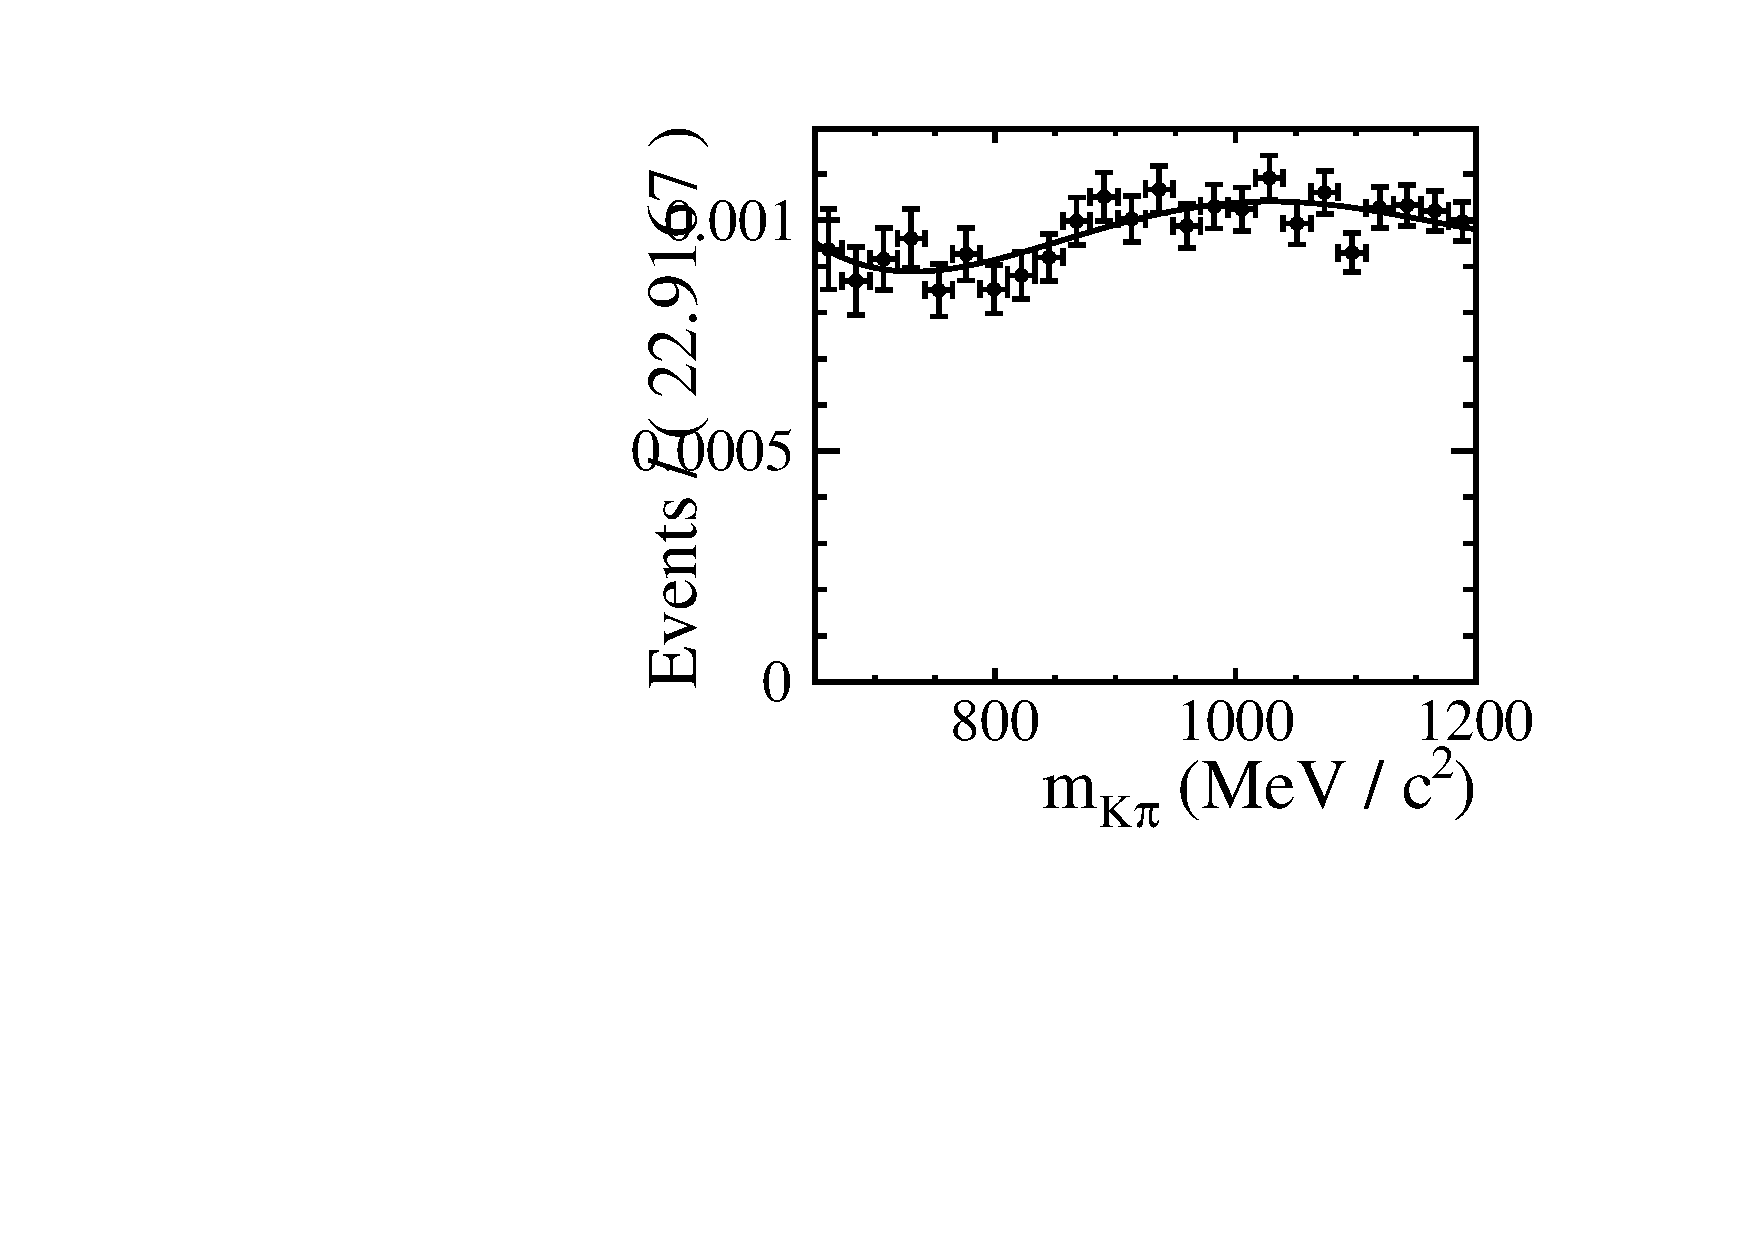
\includegraphics[width=0.48\columnwidth,page=1]{chapter7/figs/ac/fitplots.pdf}}
%\includegraphics[width=0.48\columnwidth,page=2]{chapter7/figs/ac/fitplots.pdf}
%\caption{ The efficiency as a function of \psq for phase space simulated \BdToKpimm events.
%The efficiency is parametrised by a fourth-order Chebychev polynomial. ~\label{fig:swave:ac:psq} }
%\end{figure}
%The uniformity of the efficiency was tested by fitting a fourth order Chebychev polynomial to the simulation,
%\begin{align}
%P(\mkpi; a_0, a_1, a_2, a_3)
%\end{align}
%where $a_i$ is the coefficient for the $n^{th}$ power.
%The values of the higher order coefficients were found significantly non-zero indicating that there is some curvature in the efficiency.
%
%\subsubsection{Efficiency for \qsq and \ctk}
%
%The efficiency as a function of \qsq and \ctk in the P-wave is explored in Section~\ref{sec:kstmm:ac}.
%The efficiency as a function of \ctk at low and high \qsq for phase space simulated events is shown in Fig.~\ref{fig:pwave:ctkeff}.
%\begin{figure}[tbp]
%\centering
%\subfigure[]{\includegraphics[page=5,width=0.48\columnwidth]{chapter7/figs/ac/fiteff_results_39_sysnf_0_pdfs.pdf}}
%\subfigure[]{\includegraphics[page=35,width=0.48\columnwidth]{chapter7/figs/ac/fiteff_results_39_sysnf_0_pdfs.pdf}}
%\caption{ The efficiency as a function of \ctk for the \qsq between 
%(a) 2.0 and 2.5 \gevgevcccc and (b) 17.0 and 17.5 \gevgevcccc.
%The efficiency is fitted with a fourth order Chebychev polynomial (the \textcolor{blue}{blue} curve) showing the parametrised efficiency in each \psq bin. 
%~\label{fig:pwave:ctkeff} }
%\end{figure}
%The efficiency is correlated between \qsq and \ctk such that there is a lower efficiency at large \ctk values in the low \qsq region.
%In order to have enough statistics to accurately measure the \ctk efficiency in the low \qsq region, the phase space sample was binned in 40 bins 
%of \qsq between 0.0 and 20.0 \gevgevcccc with each bin having a width of 0.5\gevgevcccc.
%
%\subsubsection{Event weighting}
%
%The event-by-event acceptance correction for the \BdToKpimm events is given by the values for the 
%polynomial fitting to the \ctk distribution in the chosen bin in \psq,
%\begin{align}

%\epsilon(\psq,\qsq,\ctk) = S(\qsq|_{\mathrm{min}\qsq}^{\mathrm{max}\qsq})\times P_i(\ctk; c_1, c_2, c_3, c_4) , \quad i \in [0,40)
%\end{align}
%and the weight of each event to correct for the acceptance is given by the inverse efficiency, 
%\begin{align}
%\omega(\qsq,\mkpi,\ctk) = 1 / \epsilon(\qsq,\mkpi,\ctk) \, .
%\end{align}
%
%\subsection{Validation}
%
%The acceptance correction can be checked to first order by comparing the distribution of re-weighted events 
%to the expected distribution of events at generator level
%Following the method in Section~\ref{sec:kstmm:ac}, the selected simulation used to calculate $S(\psq,\qsq,\ctk)$ and 
%as re-weighted and compared to the distribution of generator level events used to calculate $G(\psq,\qsq,\ctk)$.
%The distributions of simulation can be seen in Fig.~\ref{fig:swave:ac:validation}.
%\begin{figure}[tbp]
%\centering
%\subfigure[]{\includegraphics[width=0.32\columnwidth,page=2]{chapter7/figs/ac/validation_ac_1D.pdf}}
%\subfigure[]{\includegraphics[width=0.32\columnwidth,page=3]{chapter7/figs/ac/validation_ac_1D.pdf}}
%\subfigure[]{\includegraphics[width=0.32\columnwidth,page=5]{chapter7/figs/ac/validation_ac_1D.pdf}}
%\caption{ The efficiency as a function of (a) \mkpi, (b) \qsq and (c) \ctk for phase space simulated \BdToKpimm events.
%The generator level distribution is shown in black, the distribution of candidates after selection in \textcolor{red}{red}
%and the re-weighted candidates are shown in \textcolor{blue}{blue}. ~\label{fig:swave:ac:validation} }
%\end{figure}
%
%\begin{itemize}
%\item \emph{[DISCUSS]}
%\item I think you somehow have to state here that your check demonstrates that you correctly recover the distribution in he simulation. However, it is not a check of this on data (but the validation of the simulation takes care of that).
%\end{itemize}



